\section{Clustering~\label{sec:def_clustering}}

\subsection{Definition and Examples}

The clustering aim to group items such that the most similar items are in the same group.
These groups of similar items are called clusters.

Example~\ref{ex:clustering} show the clustering task for 2D points.
The points are grouped according to their distance.

For the case of authorship clustering, finding the authorship function can be useful (Definition~\ref{def:authorship} in Section~\ref{sec:definitions}).
But this task can be hard since the real author (ground truth labels) are generally not available.
Without example, finding the authorship function is not possible.

For the authorship clustering, we only aim to group similar texts instead of finding the actual authors.
This task can be solved by finding the relevant set (Definition~\ref{def:relevant_set} in Section~\ref{sec:definitions}).

To find clusters from the relevant set, a simple method is to:
Consider each pair of documents in the relevant set as: \textit{in the same cluster}.
The clusters are created using transitivity.

One main issue arise with this method.
If the relevant set is not perfect (documents pairs with actual different authors are in the relevant set), the two authors will be in the same cluster.
Noisy relevant set can quickly considered every document in a single cluster with this method.

Chapter~\ref{sec:clustering} will introduce and evaluate methods using rank lists to create the clusters instead of the relevant set.

\begin{example}
    \centering
    \caption{Clustering with 2D points}
    \label{ex:clustering}

    \begin{subexample}{\linewidth}
      \centering
      \subcaption{Unlabeled data, each point represent a sample}
      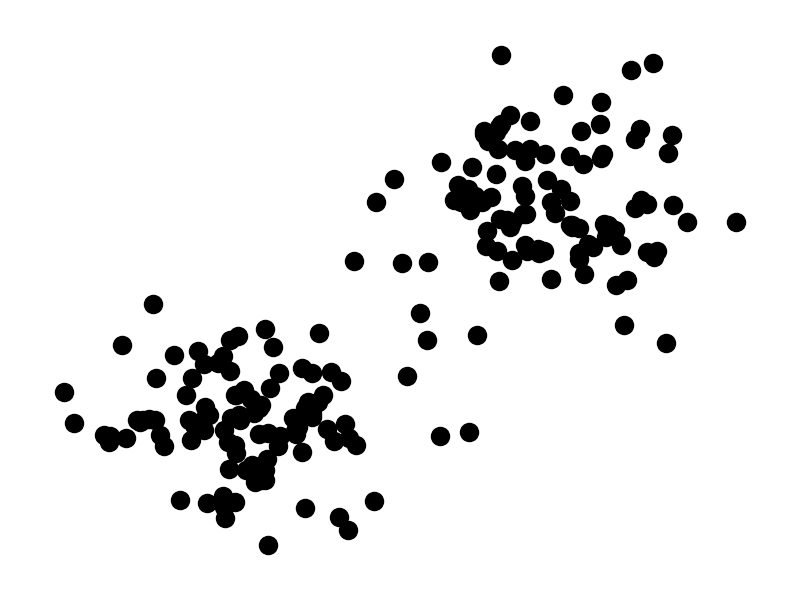
\includegraphics[width=0.9\linewidth]{img/clustering_example_1.png}
    \end{subexample}

    \vspace{0.5cm}

    \begin{subexample}{\linewidth}
      \centering
      \subcaption{A possible good clustering result, each color represent a cluster}
      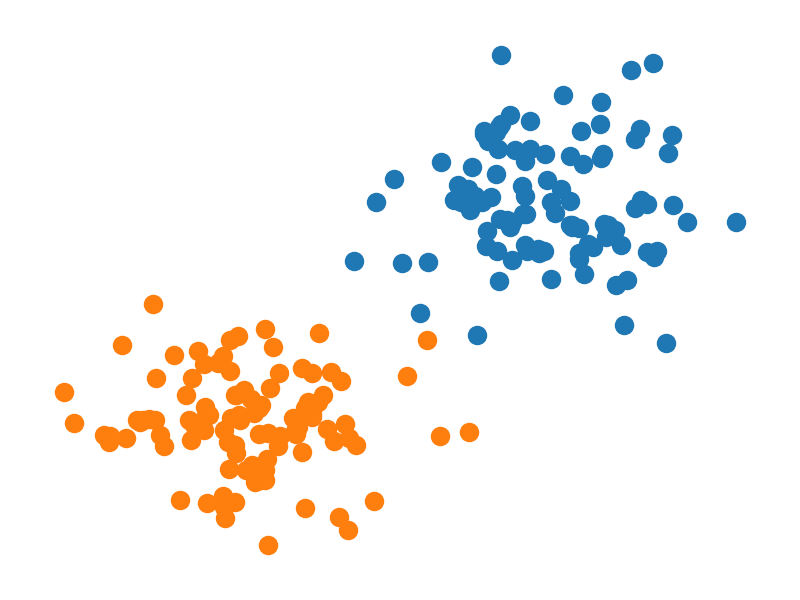
\includegraphics[width=0.9\linewidth]{img/clustering_example_2.png}
    \end{subexample}
\end{example}

\subsection{Clustering Evaluation Metrics \label{sec:clustering_evaluation_meterics}}

The methods introduced in this section are to evaluate and compare clustering models.
Therefore, the ground truth labels are required.
The metrics used are from the BCubed family (also called $B^3$, in this report) \cite{bcubed}.

BCubed has shown to satisfy the four following important constraints when evaluating clusterings \cite{bcubed}~:

\begin{enumerate}
  \item
  \textit{Cluster Homogeneity}: different authors should be in the different clusters.
  \item
  \textit{Cluster Completeness}: same authors should belong to the same cluster.
  \item
  \textit{Rag Bag constraint}: noisy or miscellaneous authors should be in the same cluster and not in \textit{healthy} clusters.
  \item
  \textit{Cluster size vs quantity constraints}: favor large clusters.
\end{enumerate}

These metrics are used to evaluate the clustering task during the PAN @ CLEF competitions~\cite{pan16}.
In addition to the BCubed family, this study introduce the \textit{cluster difference}, a simple metric to evaluate the clustering results.

\begin{definition}[Correctness~\cite{bcubed}]
  The $BCubed$ metric family is based on the following \textit{Correctness} principle.
  Let L(e) and C(e) be the author and the cluster of an element e (an element is document in the case of authorship clustering).
  The Correctness is following the biconditional condition on the author and cluster equality.
  \begin{gather*}
    \mathrm{Correctness}(e, e') = \\
    \begin{cases}
      1, & \mathrm{if} (L(e) = L(e')) \Longleftrightarrow (C(e) = C(e'))\\
      0, & \mathrm{otherwise}
    \end{cases} \\
    \mathrm{biconditional}: A \Longleftrightarrow B \equiv (A \land B) \lor (\neg A \land \neg B)
  \end{gather*}
  In other terms, the correctness has a value of 1 (100\% correct) if the two elements both are in the same cluster and have the same author OR are both in a different cluster and have a different author.
\end{definition}

\begin{definition}[$BCubed$ Precision~\cite{bcubed}]
  The $BCubed$ Precision correspond to the correctness average for all elements on the average of all element such that \textbf{their clusters are the same}.
  \begin{gather*}
    B^3_{precision} = \mathrm{avg}_{e}[\mathrm{avg}_{e' C(e)=C(e')}[\mathrm{Correctness}(e, e')]]
  \end{gather*}
\end{definition}

\begin{definition}[$BCubed$ Recall~\cite{bcubed}]
  The $BCubed$ Recall correspond to the correctness average for all elements on the average of all element such that \textbf{their authors are the same}.
  \begin{gather*}
    B^3_{recall} = \mathrm{avg}_{e}[\mathrm{avg}_{e' L(e)=L(e')}[\mathrm{Correctness}(e, e')]]
  \end{gather*}
\end{definition}

\begin{definition}[$BCubed$ $F_1$ Score~\cite{bcubed}~\cite{wiki_f1}]
  $BCubed$ $F_1$ Score uses the $F_{\beta}$ metric with $\beta = 1$.

  \begin{gather*}
    F_\beta = (1 + \beta^2) \cdot \frac{\mathrm{precision} \cdot \mathrm{recall}}{(\beta^2 \cdot \mathrm{precision}) + \mathrm{recall}}.
  \end{gather*}

  The $BCubed$ $F_1$ Score is thus computed the following way.

  \begin{gather*}
    B^3_{F_1} =
    2 \cdot \frac{B^3_{precision} \cdot B^3_{recall}} {B^3_{precision} + B^3_{recall}}
  \end{gather*}
\end{definition}

\begin{definition}[Cluster difference]
  This metric aim to evaluate if the clustering model have found the right number of cluster.
  The cluster difference is the number of cluster found $p$ minus the actual number of cluster $k$ (number of distinct authors in the corpus).
  \begin{gather*}
    Cluster_{diff} = p - k
  \end{gather*}
  A positive value indicates an overestimation of the real number of cluster, a negative value indicate the underestimation.
  Zero indicate that the right number of cluster was found.

  This value can also be used to summarize if the $B^3_{recall}$ is greater or not than the $B^3_{precision}$.
  A positive Cluster diff should indicate a larger $B^3_{precision}$ than $B^3_{recall}$, and vice versa.

  This value can be normalized by the number of documents N, which correspond to the difference of the r ratios.
  This is useful when comparing corpora results with different number of clusters.
  \begin{gather*}
    r_{diff} = \frac{p}{N} - \frac{k}{N} = \frac{p - k}{N}
  \end{gather*}
  As stated in the PAN16 evaluation campaign paper, estimating correctly the number of clusters and the r ratio is a first step to produce a good clustering~\cite{pan16}.
\end{definition}
